\chapter{Geschäftsvorfall}
\label{chap:vorfall}
Im Folgenden wird mit dem \gls{erp}-System ERPNext ein vorher festgelegter Geschäftsvorfall durchgeführt. \\
Um es so nah wie möglich an einem realen Unternehmen zu halten, wurde exemplarisch die fiktive \emph{Allgold Premium Molkerei GmbH} gewählt. Diese stellt im Allgäu bereits in dritter Generation hochwertige Molkereiprodukte her. Besonders bekannt ist sie für ihren wohlschmeckenden jungen Gouda.\\
Genau dieser soll auch im einem ausführlichen Geschäftsprozess hergestellt werden. Dafür haben wir uns für den gängigen Dreischritt \emph{Einkauf - Fertigung - Vertrieb} entschieden (\vgl Abbildung \ref{fig:geschVorfall}). Während der Durchführung werden auch an manchen Stellen Punkte angesprochen, die beim Experimentieren mit dem System besonders positiv oder negativ aufgefallen sind.
\begin{figure}[H]
  \centering
  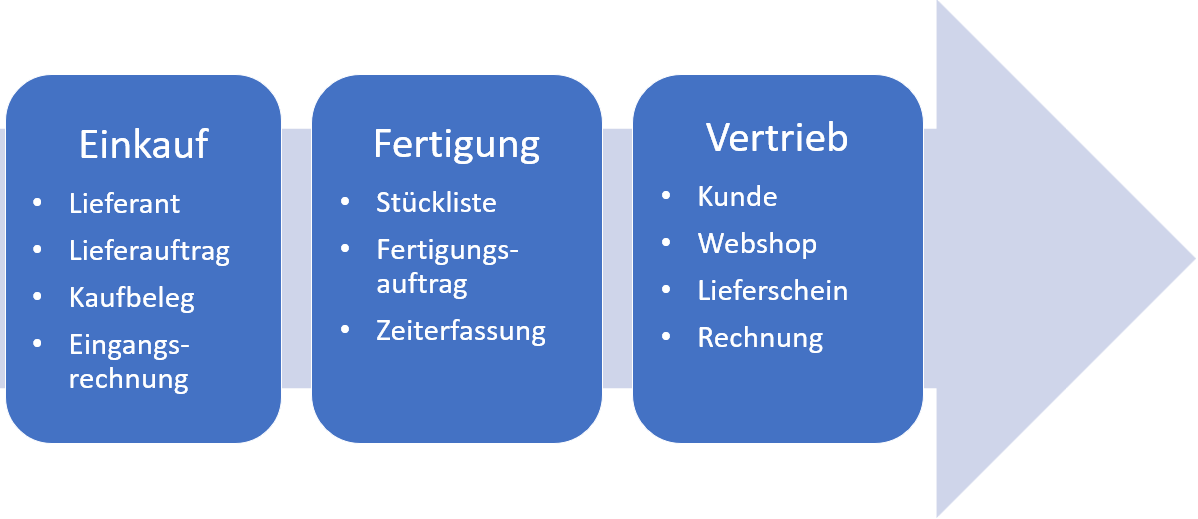
\includegraphics[width=\textwidth]{Bilder/Geschaeftsvorfall.PNG}
  \caption{Übersicht Geschäftsvorfall}
  \label{fig:geschVorfall}
\end{figure}
\emph{Hinweis:} Da die Vielzahl an Bildern zum Prozess den Rahmen dieser Seminararbeit sprengen würde, sind diese im Anhang zu finden. An den jeweiligen Stellen sind selbstverständlich diesbezüglich Verweise zu finden.

\section{Einkauf}
Da bei den einzelnen Abschnitten des Geschäftsprozesses nicht jeder kleinste Teil gezeigt werden kann, wurden bereits Vorkehrungen getroffen. So ist der Lieferant und die Rohprodukte Milch und Lab, sowie das Fertigprodukt Gouda bereits angelegt und mit entsprechenden Einkaufspreisen und Parametern versehen. Somit kann auf die anderen Prozessschritte und die Auffälligkeiten tiefer eingegangen werden.

\subsection{Lieferantenauftrag anlegen}
Zu Beginn dieses Prozesses muss für die Herstellung des Goudas Milch eingekauft werden. Mit einem neuen Lieferanten, Bauer Anton, haben wir uns im Vorfeld auf eine Lieferung von 2000 Litern Milch geeinigt. Da dieser Geschäftspartner bereits im System angelegt ist, kann beim Lieferantenauftrag mit diesem Datensatz eine Verknüpfung hergestellt werden (\vgl Abbildung \ref{fig:liefAuftrag}). Weil auch der Artikel Milch schon vorher eingepflegt worden ist, und hierbei ein Standardeinkaufspreis von 50 Cent eingetragen wurde, wird uns hier für 2000\ell\ Milch ein Gesamtbetrag von 1000€ vorausberechnet. Natürlich kann an dieser Stelle der Stückpreis individuell abgeändert und die Summe vom System dementsprechend ausgerechnet werden. \\
Klickt man auf das kleine Dreieck ganz rechts des Artikels wird dem Benutzer eine Art Detailansicht angezeigt (\vgl Abbildung \ref{fig:auftrDetail}). Dort kann er noch einige Einstellungen tätigen, die sonst von den Standardeinstellungen ersetzt werden würden. \\
Nützlich ist allgemein auch, dass man stets einfach zu verknüpften Einträgen springen kann. Dazu muss lediglich der kleine Pfeil in jenem Eingabefeld gedrückt werden, in dem man sich gerade befindet (\vgl Abbildung \ref{fig:verlArtikel}).\\
Sieht man sich den Screenshot einmal genauer an, erkennt man an manchen Stellen schlechte oder nicht vorhandene Übersetzungen, wie beispielsweise bei\ \glqq Get last purchase rate\grqq. Diese Vorkommnisse häufen sich und decken sich mit dem, was die offizielle Übersetzungsseite preis gibt (\vgl \cite{ERPNextTranslate}). Nur etwas mehr als die Hälfte der Strings der deutschen Übersetzung wurden verifiziert. Der andere Teil ist entweder maschinell übersetzt, oder wird in der Software noch im englischen Original angezeigt. \\
Wird der Auftrag nun abgeschlossen, muss der Lieferant natürlich auch über den Auftrag informiert werden. Dazu wird automatisch ein Popup-Fenster eingeblendet, sobald auf buchen gedrückt wird. Dort kann eine E-Mail versendet werden, inklusive des Auftrags in PDF-Form (\vgl Abbildung \ref{fig:auftrPdf}). Dies erfordert die Einrichtung einer geeigneten Mail-Adresse in den Einstellungen, über die dann die Benachrichtigungen verschickt werden können.

\subsection{Ware empfangen}
Nach dem Absenden eines Lieferantenauftrages und der Bearbeitung seitens des Lieferanten kommt natürlich auch der Zeitpunkt, zu dem die Ware im Unternehmen eintrifft. Um eine Aktion im Rahmen des getätigten Lieferantenauftrags zu unternehmen, muss man diesen einfach in der Auftragsübersicht auswählen. Dort bekommt man dann direkt die häufigsten Aktionen vorgeschlagen (\vgl Abbildung \ref{fig:auftrUebersicht}). Oben links wird durch Ampelfarben und Text, wie hier bei \glqq Um zu empfangen und abzurechnen\grqq\ stets der aktuelle Stand des Lieferantenauftrags angezeigt. Das sieht man auch weiter unten beim Artikel Milch, der gelb gefärbt ist, was in diesem Kontext bedeutet, dass er noch nicht im Lager gebucht ist.\\
Um nun den Erhalt der Ware zu bestätigen und auf das vorher festgelegte, oder ein anderes Lager zu buchen, muss auf das Plus-Zeichen neben Kaufbeleg gedrückt werden. Dadurch werden die bereits vorhandenen Informationen direkt in die nächste Maske übernommen (\vgl Abbildung \ref{fig:kaufbeleg}). Ein einfacher Klick auf den Text Kaufbeleg würde lediglich alle offenen Kaufbelege zu diesem Lieferantenauftrag anzeigen. \\
Sollte die angenommene Menge kleiner sein als die Bestellmenge, also nur eine Teillieferung erfolgt sein, kann das über den Kaufbeleg umgesetzt werden. Auch hier gilt wieder: Ein Klick auf das kleine Dreieck bietet dem Benutzer mehr Einstellungsmöglichkeiten. Nach dem Speichern des Kaufbelegs werden nicht ausgefüllte Felder, oder nicht erledigte Tätigkeiten von der Software hervorgehoben. Da die Molkerei stets die frische ihrer Produkte und einwandfreie Rohstoffe garantiert, wurde im Vorfeld beim Rohmaterial Milch ein Häkchen für eine Qualitätskontrolle bei Wareneingang gesetzt. Deshalb fordert das System auf, diese durchzuführen (\vgl Abbildung \ref{fig:mittQual}). An dieser Stelle wird ein neuer Benutzer der Systems wahrscheinlich erst einmal etwas irritiert sein, da nicht sofort ersichtlich ist, durch welche Schaltfläche diese Kontrolle angestoßen werden kann. Dafür muss nämlich wieder in die Detailansicht (= kleines Dreieck) des betreffenden Artikels gewechselt werden. Dort existiert dann im Abschnitt Lager und Referenz ein dementsprechender Punkt. Das System schlägt dem Benutzer an geeigneter Stelle stets schon vorhandene Elemente vor (soweit existent), oder lässt direkt ein neues Element anlegen, ohne dass der User aus der aktuellen Maske ins Hauptmenü springen muss (\vgl Abbildung \ref{fig:auswQual}). \\
Die Qualitätskontrolle selbst (\vgl Abbildung \ref{fig:qualPruef}) ist schnell geschehen, da die Molkerei nur den Gehalt von Antibiotika in der Milch prüft. Danach lässt sich der Kaufbeleg ohne weitere Probleme buchen. \\
Geht man nun auf den Lieferantenauftrag zurück, fällt auf, dass sich der Status oben links auf \glqq Abrechnen\grqq\ geändert hat. Über das Plus bei Eingangsrechnung kann nun auch diese hinzugefügt werden. Im Lieferantenauftrag wechselt der Status danach auf \glqq Abgeschlossen\grqq\, aber die Lieferung ist noch unbezahlt. Der User könnte nun eine Zahlung über den Lieferantenauftrag anlegen, jedoch würde dabei der Bezug zur Rechnung verloren gehen. Geht man nun über die Verlinkung (\vgl Abbildung \ref{fig:auftrUebersicht}) in die Eingangsrechnung des Auftrags und führt diese durch, wird ebendiese Verknüpfung vom System selbstständig hergestellt (\vgl Abbildung \ref{fig:zahlung}). Danach ändert sich der Status auf grün und \glqq Bezahlt\grqq. So bleibt die Zahlung auch später besser zuordenbar und Rechnungen bleiben nicht unabsichtlich unbezahlt.

\section{Fertigung}
Auch beim Bereich Fertigung wurden im Vorfeld bereits einige Dinge für die Stückliste angelegt. Dazu zählt der Arbeitsgang \glqq Lab hinzufügen\grqq\ (\vgl Abbildung \ref{fig:arbGang}) mit dem Arbeitsplatz \glqq Kessel\grqq\ (\vgl Abbildung \ref{fig:arbPlatz}).

\subsection{Stückliste anlegen}
Um den Gouda der \emph{Allgold Premium Molkerei GmbH} herzustellen wird eine Stückliste benötigt (\vgl Abbildung \ref{fig:stListe}). Diese kann neben benötigter Materialien auch Arbeitsgänge beinhalten. In diesem Beispiel verwenden wir zehn Liter Milch, sowie eine Einheit Lab. Dazu kommt ein Arbeitsgang, bei dem das Lab zu der Milch in den Kessel geschüttet wird. Aufgrund mangelnder Expertise unsererseits bei der Käseherstellung soll dies für den Moment schon genügen. \\
Bei dieser Stückliste wird automatisch ein Häkchen für den Standard gesetzt. Dies wird auch so belassen, damit die neue Stückliste später automatisch ausgewählt wird. 
Etwas unübersichtlich ist hierbei, dass die \glqq Operation Time\grqq\ für den Arbeitsgang in Minuten und nicht in Stunden angegeben werden muss. Dies sieht man erst, wenn man in die Detailansicht eines Arbeitsganges wechselt. Verwechselt man das unabsichtlich, könnten die Betriebskosten vollkommen verfälscht werden. \\
ERPNext bietet zudem noch eine Möglichkeit, um eventuell anfallenden Ausschuss beziehungsweise Abfall bei der Herstellung zu berücksichtigen. Da dies aber bei diesem Beispiel nicht der Fall sein wird, kann das getrost übersprungen werden.

\subsection{Fertigungsauftrag erstellen}
Anhand der Stückliste kann nun ein Fertigungsauftrag für Gouda erstellt werden (\vgl Abbildung \ref{fig:fertAuftr}). Trägt man den zu fertigenden Artikel ein, wird automatisch die Standardstückliste zu diesem Artikel ausgewählt. Auch mehrstufige Stücklisten sind hierbei möglich, um diese Arbeit aber in einem überschaubaren Rahmen zu halten, wurde darauf verzichtet und auf eine normale Baukastenstückliste zurückgegriffen. \\
Beim Eintrag der herzustellenden Menge werden anhand der gewählten Stückliste die erforderliche Mengenanzahl der einzelnen Artikel, sowie die benötigte Zeit für die Arbeitsgänge ermittelt. Daraus ergeben sich dann für den Arbeitsgang auch die geplanten Betriebskosten.
An und für sich sind Pflichtfelder stets durch einen gelben Hintergrund gekennzeichnet. Beim Speichern und Buchen fällt dann jedoch auf, dass hier auch zwei Lagerplätze eingetragen werden müssen, welche diese Kennzeichnung davor nicht getragen haben. Das Eingangslager ist für die fertigen Erzeugnisse notwendig und das Fertigungslager dementsprechend für die Lagerung während der Fertigung. Danach lässt sich der Fertigungsautrag ohne Probleme ins System einbuchen und dessen Status wechselt auf \glqq Nicht begonnen\grqq\ (\vgl Abbildung \ref{fig:fertNichtBeg}). Im gleichen Augenblick wird ein dazugehöriges Timesheet erstellt.

\subsection{Zeiterfassung pflegen}
Nun muss die Produktion gestartet und die entsprechenden Materialien aus dem Lager transferiert werden (\vgl Abbildung \ref{fig:matTransfer}). Dabei könnte auch nur eine Teilmenge hergestellt werden, was wir in diesem Beispiel jedoch nicht tun werden. Alle benötigten \glqq Einzelteile\grqq\ sind verfügbar und können somit verschoben werden (\vgl Abbildung \ref{fig:lagBuchung}). Nach Beendigung des Fertigungsauftrages, mit dem von uns erdachten Arbeitsgang, kann die benötigte Zeit ins System eingebucht werden (\vgl Abbildung \ref{fig:timeSheet}). Dabei wird zuerst die veranschlagte Zeit voreingetragen. Sollte der Mitarbeiter mehr oder weniger Zeit benötigt haben, könnte er das an dieser Stelle abändern. Das hätte dann wiederum Einfluss auf die Kosten des Arbeitsgangs und somit des Herstellungspreises unseres Goudas. In diesem Beispiel werden alle Tätigkeiten mit einem administrativen User durchgeführt. In der Realität wäre das natürlich nicht der Fall und so könnten auch Auswertungen des Controllings anhand der gebuchten Zeiten erstellt werden. \\
Ist unser Gouda gefertigt, muss eine neue Lagerbuchung angestoßen werden, um die Roh-Artikel aus dem Lager zu nehmen und den Gouda ins Lager der Fertigerzeugnisse zu legen (\vgl Abbildung \ref{fig:beenFertig}).

\section{Vertrieb}
Für den Vertrieb des Goudas  hat ERPNext nicht nur die Möglichkeit Kunden über das \gls{erp}-System durch einen Mitarbeiter der Molkerei anzulegen, sondern auch den Bestellprozess direkt durch den Kunden über einen Webshop anzustoßen. Dadurch wird das System direkt zur Verkaufsplattform.\\
In diesem Szenario will der Kunde \glqq Großhandel Gummersbach\grqq\ Gouda für sein Geschäft einkaufen.

\subsection{Kunden anlegen}
Der Kunde kann sich unter dem Reiter \glqq Anmelden\grqq\ der Webseite einen neuen Account anlegen. Dazu muss er seinen vollständigen Namen (bzw. den Namen des Geschäfts), sowie eine E-Mail-Adresse angeben (\vgl Abbildung \ref{fig:regKunde}). Dadurch kommt er nie mit der Verwaltungsplattform, wie sie ein Mitarbeiter benutzt, in Berührung. Nach erfolgreicher Registrierung wird dem Kunden eine E-Mail zugeschickt (\vgl Abbildung \ref{fig:regMail}). Nach Setzen eines Passworts kann auch schon im Webshop eingekauft werden. \\ 
Zu diesem Zeitpunkt ist bereits ein neuer Kundeneintrag in ERPNext generiert worden und für Mitarbeiter sichtbar.

\subsection{Verkaufsauftrag erstellen}
In herkömmlichen Webshops können gleich mehrere Einheiten desselben Produktes auf einmal ausgewählt werden. Das ist mit dem Webshop von ERPNext nicht möglich (\vgl Abbildung \ref{fig:webGouda}). Erst im Einkaufswagen können mehrere Einheiten ausgewählt und ausgecheckt werden (\vgl Abbildung \ref{fig:webChart}). Vor dem Absenden der Bestellung wird noch eine Rechnungs- und Lieferadresse benötigt (\vgl Abbildung \ref{fig:webWarenkorb}). Nach dem Aufgeben der Bestellung hat der Kunde dann noch die Möglichkeit, den Auftrag auszudrucken.

\subsection{Zahlung tätigen}
Nach dem Eingang des Kundenauftrags in das System hat nun die Rechnungsstellung und Bezahlung zu erfolgen. Die Rechnung ist schnell erstellt und kann wieder per E-Mail an den Kunden inklusive persönlicher Nachricht übermittelt werden. \\
Danach kann die Zahlung erfolgen. Eigentlich wäre es an sich sinnvoller, diese direkt beim Bestellvorgang abzuwickeln. Dafür fehlt lediglich ein Payment-Gateway, dass die Bezahlung per Kreditkarte o.ä. gegen eine Gebühr erlaubt. Das kann durch die Zahlungseinstellungen im \gls{erp}-System relativ einfach realisiert werden. Dazu stellt ERPNext schon vorgefertigte Schnittstellenanbindungen zu Stripe, PayPal und dem indischen Dienstleister Razorpay zur Verfügung. \\
Wir wollen unsere Bestellung aber auf die gebräuchliche Art, per Überweisung, bezahlen. Dazu wird über den Kundenauftrag eine neue Zahlung erzeugt und mit den dementsprechenden Parametern gefüllt (\vgl Abbildung \ref{fig:zahKunde}). Dabei fällt auf, dass die ursprüngliche Zahlung von 11,40€ auf 11€ abgerundet wurde. Das scheint eine spezielle Einstellung zu sein, die jeweils immer auf den vollen Euro abrundet. Für andere Währungssysteme mag dies Sinn ergeben, jedoch ist das im Euro-Raum so nicht gebräuchlich. \\
Der Kunde kann stets den aktuellen Status seiner Bestellung über seinen Zugang zum Webshop einsehen. Bei erfolgter Bezahlung wechselt dieser zum Beispiel auf \glqq Bezahlt und nicht ausgeliefert\grqq. 

\subsection{Ware ausliefern}
Die Auslieferung der angeforderten Ware ist der letzte Teil dieses Geschäftsprozesses. Dafür muss der Benutzer beim Kundenauftrag einen Lieferschein erstellen. An dieser Stelle wurde eine kleine Anpassung programmiert (\vgl Abbildung \ref{fig:jsPopup}). Per JavaScript kann clientseitig Code in die Anwendung integriert werden. Im Normalfall ist dies eher für Formulare, beispielsweise bei der Berechnung von Werten gedacht, nichtsdestotrotz kann auch ein Popup mit hilfreichen Informationen angezeigt werden. \\
Genauso wie anfangs eine Qualitätsprüfung beim Eingang der Milch eingestellt wurde, muss nun die Qualität auch beim Ausgang des Endproduktes Gouda geprüft werden. Dazu muss diese Qualitätsprüfung auf dem weiter oben bereits erklärten Weg hinzugefügt werden. Hierbei muss für die Buchhaltung auch ein Aufwands- und Ertragskonto für den zu verbuchenden Betrag eingetragen werden. \\
Der zuvor hergestellte Gouda hat zudem die Besonderheit, dass er für eine bessere Zurückverfolgbarkeit über eine Chargennummer verfügt. Mit dieser Funktionalität müssen so beispielsweise bei einer Rückrufaktion nur die betroffenen Chargen und nicht alle Produkte geprüft werden. \\
Mit abschließender Buchung des Lieferscheins ist der gesamte Prozess von Einkauf bis Vertrieb abgeschlossen.

\section{Fazit}
Durch das Erarbeiten dieses Geschäftsprozesses und das Experimentieren mit dem System lässt sich gut ein abschließendes Resümee ziehen. \\
Insgesamt ist ERPNext sehr gut und angenehm zu benutzen. Durch das den mobilen Plattformen entledigte Design findet man sich sehr schnell intuitiv zurecht. Das Design lässt sich auch von dem anfangs vorgegebenen Lila, passend zur Farbe des ERPNext-Logos, sehr leicht auf das firmeneigene Corporate Design anpassen. Es gibt allgemein viele Einstellungen, um den jeweiligen Bedürfnissen der Anwender gerecht zu werden. Dazu zählen auch automatisierte Workflows, die der ein oder andere User schon von Programmen wie Microsoft Sharepoint kennen könnte. Will man tiefergreifendere Anpassungen machen, ist dies mit ein wenig Code auf Client- wie auf Serverseite möglich. Dazu existiert auch eine Entwickler-Dokumentation, sowie integrierte Hilftexte und -videos im \gls{erp}-System. \\
Die Navigation zwischen den einzelnen Bereichen gestaltet sich durch die Verlinkungen mittels der Pfeilchen sehr einfach. Wo Verknüpfungen existieren, ist es immer möglich in andere Bereiche zu wechseln, ohne den Umweg über das Hauptmenü nehmen zu müssen. Dort wo in Übersichten, wie beispielsweise dem Lieferantenauftrag, verwandte Formulare befüllt werden müssen, eignet sich das Plus-Zeichen hervorragend um die wichtigsten Parameter zu übernehmen.

Trotz alledem gibt es selbstverständlich auch Negatives zu berichten, das während dem Testen aufgetreten ist. \\
Bei der Erstellung eines Accounts oder einer Rechnung wird abschließend vom System eine E-Mail gesendet, soweit dies eingerichtet ist. Hier war beobachtbar, dass diese \emph{meist} sofort an der Zieladresse angekommen sind, aber ab und an auch manchmal einige Minuten Zeit benötigt haben. Ob dies an der zum Versenden eingesetzten Gmail-Adresse liegt, oder ob dieses Problem tiefer im System besteht, ist unklar. In diesem Szenario habenauch nur wenige Personen auf das System zugegriffen. Deshalb ist fraglich, wie es sich auf die Performance auswirkt, sollten einmal mehrere hundert Personen E-Mails über ERPNext verschicken müssen. \\
So gut die Verknüpfungen an den meisten Stellen sind, so ist es umso gravierender, wenn diese fehlen. Auf unseren Geschäftsvorfall bezogen bedeutete das beispielsweise, dass es keine Verbindung von Produkt und Lieferant gab. Somit kann man z.B. auch das Produkt Lab bei einem Bauer bestellen, der eigentlich nur Milch liefert. \\
Die Benutzerführung ist zudem nicht immer Konsistent. Meist übernimmt das Plus-Zeichen alle benötigten Werte, manchmal muss man aber für genau diese Funktionalität den Button \glqq Make\grqq\ rechts oben betätigen. Den durchschnittlichen User könnte das sehr verwirren. \\
Wie in den vorangegangenen Abschnitten zum Geschäftsvorfall bereits angesprochen sind die Übersetzungen ins Deutsche, sowie die lokalen Einstellungen nicht immer existent. Man mag meistens erahnen können, was bestimmte Floskeln bedeuten sollen, allerdings wäre eine weiter fortschreitende Übersetzung seitens der Community sehr wünschenswert. Wieso die lokalen Datumseinstellungen, sowie das lokal gebräuchliche Komma statt einem Dezimalpunkt nicht schon von vornherein eingestellt sind und seltsame Rundungsregeln angewandt werden ist sehr fraglich. Es sollte lieber keine deutsche Version existieren, solange diese nicht vollständig auf die lokalen Gegebenheiten abgestimmt ist. \\
Meistens lief das System stabil und zeigte nur geringe Latenzen beim Speichern und Buchen von Einträgen. Trotz allem gab es mehrere Systemausfälle während dem erneuten Durchgehen des Geschäftsprozesses für diese Arbeit (\vgl Abbildung \ref{fig:fehlMeldung}). Dabei stüzte ERPNext aus unbekannten Gründen ab und ließ sich auch nicht mehr durch einen Neustart der Bench initialisieren. Lediglich ein Neustart des Servers behob das Problem. Dabei wurde auch in den diversen Log-Files des Systems kein Fehler gefunden, der diesen Absturz rechtfertigen würde. Nach einiger Zeit war ERPNext auch wieder vollständig funktionstüchtig und ähnliche Probleme traten nicht mehr auf.

Zusammenfassend lässt sich sagen: Dieses \gls{erp}-System vereint gute, neue Ansätze und eine angenehm zu benutzende Oberfläche. Allerdings werden erdachte Konzepte nicht durchgehend umgesetzt und die Ausrichtung auf den deutschen Markt lässt öfter einige Anpassungen und Übersetzungen missen.